%TCIDATA{Version=5.00.0.2570}
%TCIDATA{LaTeXparent=0,0,Presentation-CAFE-displacement-subdoc.tex}
% $Id: Presentation-subdoc.tex 6886 2017-07-19 21:29:29Z lv39 $
% $URL: https://forge.cornell.edu/svn/repos/jma7/sloan-synthetic-data-server/text/Presentation/Presentation-subdoc.tex $
\section{Goal}

\begin{frame}{Providing access to confidential data: a dichotomy?}
\begin{itemize}
    \item Apply SDL methods to render data less sensitive (coarsen, sample), publish \textbf{public-use data}
    \item[ ]
    \item[ ]
\end{itemize}
\end{frame}

\begin{frame}{Public-use data process}
\includegraphics[width=\textwidth,page=3]{outputs/ContainerizedDataCycle.drawio.pdf}
\end{frame}

\begin{frame}{Providing access to confidential data: a dichotomy?}
\begin{itemize}
    \item Apply SDL methods to render data less sensitive (coarsen, sample), publish \textbf{public-use data}
    \item[ ]
    \item Provide access to confidential data directly, apply SDL methods to \textbf{outputs of models} (\textbf{RDC model})
\end{itemize}
\end{frame}

\begin{frame}{Public-use data process}
\includegraphics[width=\textwidth,page=2]{outputs/ContainerizedDataCycle.drawio.pdf}
\end{frame}

\begin{frame}{Providing access to confidential data: broadening the toolkit}
\begin{itemize}
    \item Apply SDL methods to render data less sensitive (coarsen, sample), publish \textbf{public-use data}
    \item Generate synthetic data, publish \textbf{synthetic public-use data}
    \item Provide access to confidential data directly, apply SDL methods to \textbf{outputs of models} (\textbf{RDC model})
\end{itemize}
\end{frame}

\begin{frame}{What about inference validity?}
\begin{itemize}
    \item \textbf{Public-use data}: rarely disputed, sometimes tested, occassionally fails (unions, top earnings, ...)
    \item \textbf{Synthetic public-use data}: design goal, generally high target (replace access to confidential data)
    \item \textbf{RDC model}: generally undisputed, because access is to the unmodified data
\end{itemize}
\end{frame}

\begin{frame}{What about confidentiality protection?}
\begin{itemize}
    \item \textbf{Public-use data}: old-style SDL, sometimes disputed. Known to fail for newer data (linked data, geographically precise data)
    \item \textbf{Synthetic public-use data}: design goal, generally high target (replace access to confidential data)
    \item \textbf{RDC model}: high, but at the cost of complex access mechanism
\end{itemize}
\end{frame}

\section{Synthetic Data}

\begin{frame}{Synthetic Data}
\begin{quote}
``Synthetic data are simulated data generated from statistical models.'' 
\end{quote}
{\tiny \href{http://www.census.gov/programs-surveys/sipp/methodology/sipp-synthetic-beta-data-product.html}{SSB webpage} }
\end{frame}

%\begin{frame}{Dang: Census Bureau beat me to the punch}
%	\begin{quote}
%		\href{https://www.census.gov/library/fact-sheets/2021/what-are-synthetic-data.html}{census.gov/.../what-are-synthetic-data.html}
%		\includegraphics[width=\linewidth]{../../screenshots/census-synthetic-2021-06}
%	\end{quote}
%\end{frame}

%\begin{frame}{Synthetic Data}
%	\begin{quote}
%		``... computer programming... \textbf{completely simulated}...\\
%		... statistics ... \textbf{combining data} ... to produce estimates ...\\
%		... data confidentiality ... \textbf{modeled statistical outputs} ...''
%	\end{quote}
%\end{frame}


\begin{frame}{Synthetic Data are protective}
	\begin{quote}
		``They are
		designed to protect the confidentiality of the people and firms in the underlying
		confidential data''
	\end{quote}
{\tiny \href{http://www.census.gov/programs-surveys/sipp/methodology/sipp-synthetic-beta-data-product.html}{SSB webpage} }
\end{frame}

\begin{frame}{(Partially) Synthetic Data}
	\begin{quote}
		``...all variables are synthesized, or modeled, in a way that changes the record of each individual in a manner designed to preserve the underlying covariate relationships between the variables...''
	\end{quote}
	{\tiny \href{http://www.census.gov/programs-surveys/sipp/methodology/sipp-synthetic-beta-data-product.html}{SSB webpage} }
\end{frame}



\begin{frame}{Also called ``synthetic data'':}
	\begin{block}{These are not...}
	\begin{enumerate}
		\item ``Test files'' (= synthetic data drawn from univariate distributions) (used at various statistical agencies)\\
		\item Custom-generated (bespoke) synthetic data per project   \href{http://www.lscs.ac.uk/projects/synthetic-data-estimation-for-uk-longitudinal-studies/}{SYLLS} \\{\tiny \citep{synthpop}}
	\end{enumerate}
\end{block}
\end{frame}

\begin{frame}{Variations in the data generating process}
	\begin{block}{Synthetic data can be generated in a variety of ways}
		\begin{enumerate}
			\item Drawn from univariate distributions of each variable
			\item Sampled from a posterior-predictive distribution of a particular analytical model
			\item Sampled from a posterior-predictive distribution of a model of the data 
			\item Sampled from a differentially private high-dimensional histogram
		\end{enumerate}
	This affects both analytic (or inferential) validity as well as protective properties
	\end{block}
\end{frame}


\begin{frame}{Synthetic Microdata in the Wild}
	\begin{block}{}
		\begin{itemize}
			\item \textbf{SIPP Synthetic Beta} (person-level survey + admin data) \citep{ssafinal,CreationSSBv7}
			\item \textbf{Synthetic LBD} (establishment-level data) \citep{KinneyEtAl2011}
			\item German establishment data \citep{drechsler2012}
			\item Canadian SyntheticLEAP (firm-level data) \citep{alam2020a}
		\end{itemize}
	\end{block}
\end{frame}


\begin{frame}
	\begin{block}{Synthetic Tabular Data in the Wild}
		\begin{itemize}
			\item ACS group quarters data (tabular data)
			\item OnTheMap (tabular data) \citep{Ashwin2008}
		\end{itemize}
	\end{block}
Most of these are aimed at ``inferentially valid'' applications.
\end{frame}

\begin{frame}{Quality assessment of synthetic data}
	\begin{block}{Three dimensions of assessment}
		\begin{enumerate}
			\item Inferential validity: are inferences based on synthetic data approximately the same as those drawn from unprotected data?
			\item Confidentiality protection: are the synthetic data protective of the privacy of respondents in the unprotected data?
			\item Analyst utility: are the synthetic data useful to analysts?
		\end{enumerate}
	\end{block}
\end{frame}



\begin{frame}{Datasets}
	\begin{block}{\acf{SSB}}
		\begin{itemize}
			\item 	provide access to linked data that are usually not publicly available
			% due to confidentiality concerns. 
			\begin{itemize}
			\item  mostly synthetic: all variables except two are synthesized
			\item  \textit{gender} and a \textit{link to the first reported marital partner} are the exception. 
			\item  method: estimate the joint distribution of all the variables in the data and taking random draws from this modeled distribution. %These draws are then used to replace actual data values. This process is repeated multiple times to create a set of 16 files, 
   		    \end{itemize}
			\item The goal of the SSB is to produce results that are \textit{qualitatively} the same as results from the Completed Gold Standard Files. 
			\item Method: \cite{CreationSSBv7}
			\item Codebook: \cite{CED2AR-SSBv70}
			
		\end{itemize}
	\end{block}
\end{frame}

%\begin{frame}{Datasets}
%	\begin{block}{\acf{SynLBD}}
%		\begin{itemize}
%			\item goal: provide users with access to a longitudinal business data product  without disclosing confidential information. 
%			\item based on LBD:  establishments' employment and payroll, establishments' birth and death years, and multi-unit status, conditional on industrial classification. 
%			\item Methods: \cite{MirandaJarmin2002,KinneyEtAl2011}
%			\item Codebook: \cite{CED2AR-SynLBDv2}
%		\end{itemize}
%	\end{block}
%\end{frame}

\section{Developing Synthetic Data}

\begin{frame}{Enter the Validation Server}
    \begin{itemize}
        \item Creating (general purpose) synthetic data that achieves high inferential validity and high confidentiality protection is \textbf{hard}.
        \item Target measures for known analyses/models are straightforward to achieve \citep{KinneyEtAl2011,drechsler2012,ssafinal,CreationSSBv7} and can even be achieved using \textbf{canned} procedures \citep{synthpop2016}
        \item \textbf{Broadening} the set of valid analyses is \textbf{hard} (problem of congeniality of model \citep{xiao-li-congenial})
    \end{itemize}

Approach taken: iterative approach combined with unstructured user feedback loop through validation \citep{reiterVerificationServersEnabling2009}.
\end{frame}

\begin{frame}{Validation Server}
\begin{block}{Validation}
    \begin{itemize}
        \item Researcher develops analysis in unsecure environment (using synthetic data, public-use data): $M(\Xi(D)) = M(D^*) \rightarrow Y^*$
        \item Researcher submits analysis to data publisher
        \item Data publisher runs analyis on confidential data $M(D) \rightarrow Y $
        \item Data publisher reports back 
        \begin{itemize}
            \item Quality metric $Q(Y^*,Y)$ and/or
            \item Confidentialized output from model $\Xi(Y) = Y^{'}$
        \end{itemize}
    \end{itemize}
\end{block}
    
\footnotesize In principle not restricted to synthetic data - any modified data (e.g., \textbf{public-use data}) can be ``validated'' through such a system. 
\end{frame}



    
%\begin{frame}{Streamlining}
%\includegraphics[width=\textwidth,page=2]{outputs/ContainerizedDataCycle.drawio.pdf}
%\end{frame}

%\begin{frame}{...}
%\includegraphics[width=\textwidth,page=3]{outputs/ContainerizedDataCycle.drawio.pdf}
%\end{frame}


\begin{frame}{Validation Server}
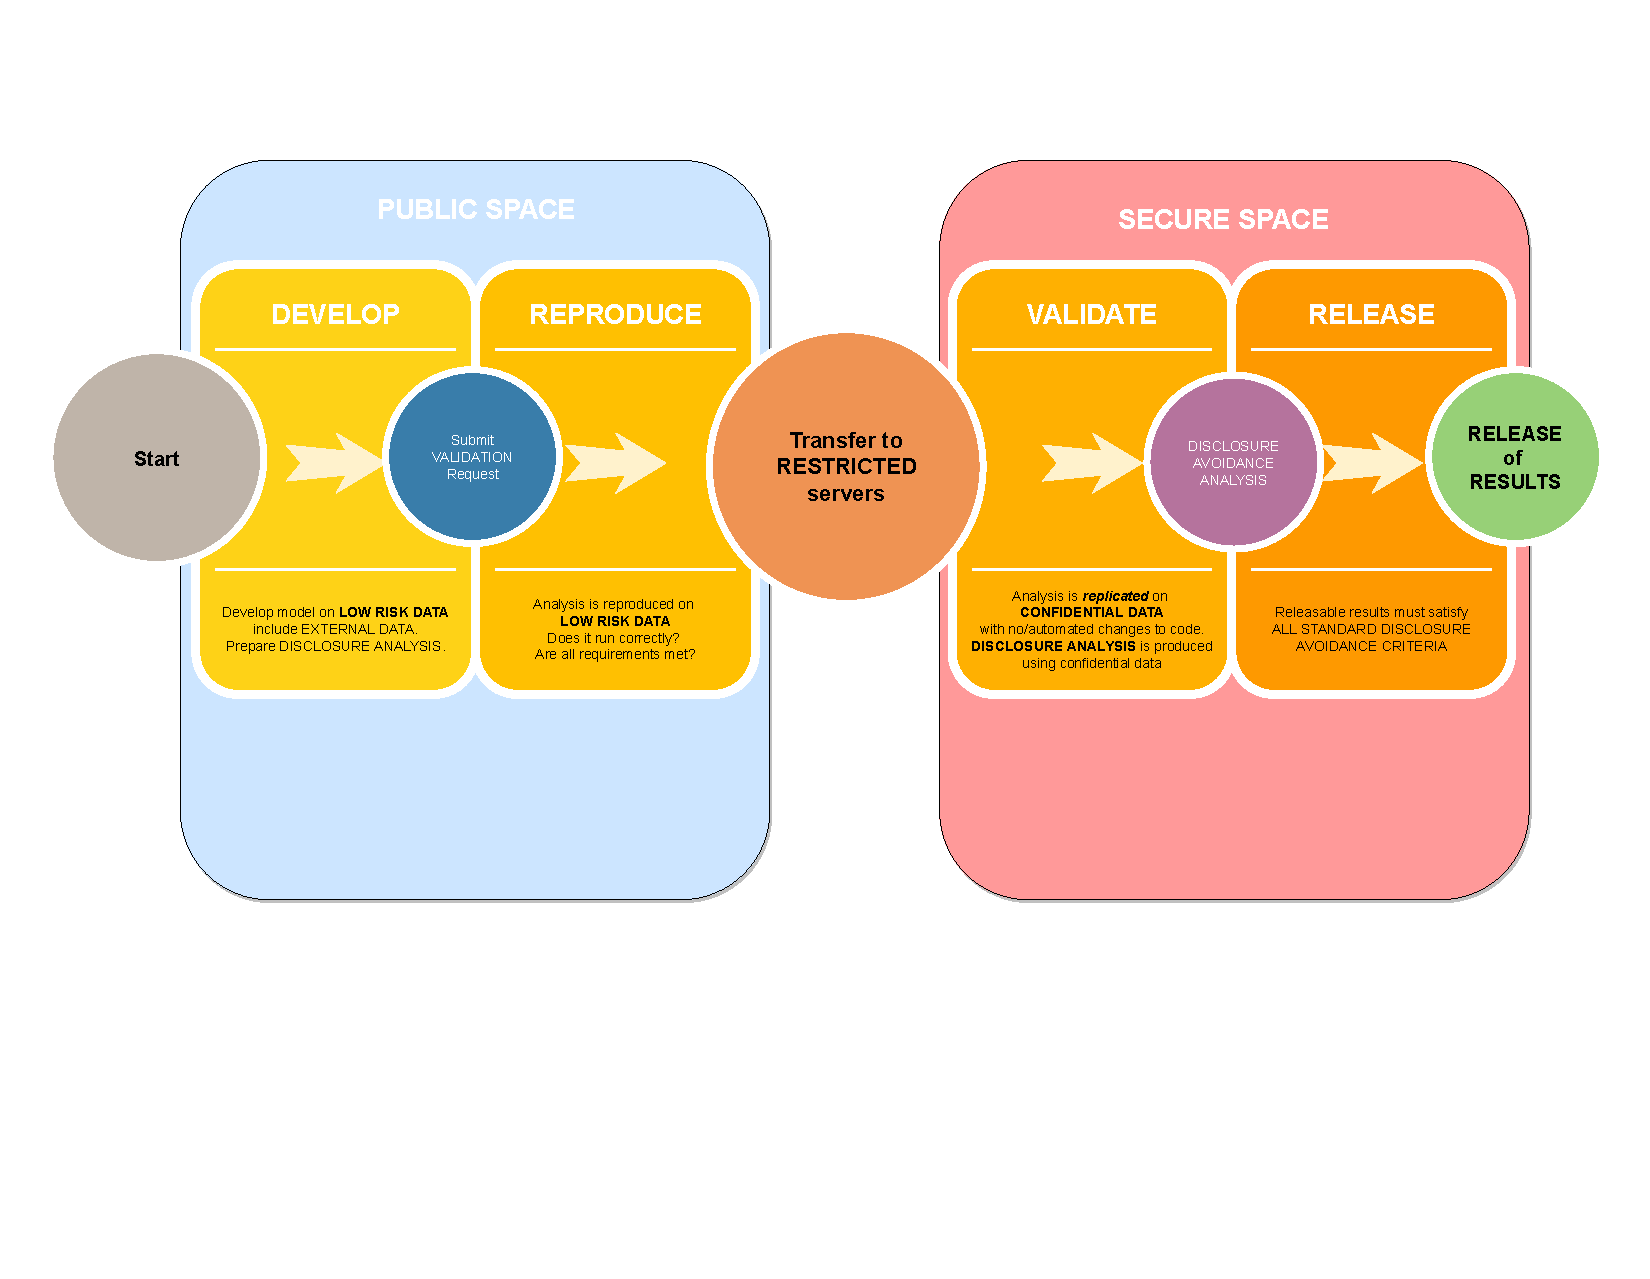
\includegraphics[width=\textwidth,page=1]{outputs/ContainerizedDataCycle.drawio.pdf}
\end{frame}

\begin{frame}{SDS Validation Server Cycle}
The \ac{SDS} was set up with the specific goal to test a mechanism to gather broad user input and improve the synthetic data iteratively.
\begin{block}{Iterate}
\begin{itemize}
    \item Make available v$(X)$ of synthetic data
    \item Provide access to researchers
    \item Allow for validation
    \item Collect models, feedback
    \item Revise synthetic data generation, prepare v$(X+1)$
\end{itemize}
\end{block}
\end{frame}

\begin{frame}{History of datasets}
	\begin{figure}[h]
		\Tree[.{SDS} 
		[.{SIPP Synthetic Beta}
		[.{v5 \textbf{2010}}
		[.{}
		[.{}
		[.{v5.1 \textbf{2013}}
		[.{}
		[.{v6.0 \textbf{2015Q1}}
		[.{}
		[.{\href{https://www2.ncrn.cornell.edu/ced2ar-web/codebooks/ssb/v/v7}{v7.0} \textbf{2018Q3}}
		]]] 
		]]]]]]
		%%%%%%%%%
		[.{SynLBD}
		[.
		[.{\href{https://www2.ncrn.cornell.edu/ced2ar-web/codebooks/synlbd/v/v2}{v2.0} \textbf{2011}}
		[.{}
		[.{v3.0-unreleased \textbf{2014}}
		[.{}
		[.{}
		[.{}
		[.{}
		[.{}
		[.{}
		]]]]]]]]]]]
		]
		%	\caption{History of dataset releases}
	\end{figure}
	
\end{frame}

\begin{frame}{SDS Validation Server Quid-pro-quo}
The \acf{SDS} embodied a quid-pro-quo between researchers and the agency.
\begin{block}{NSI}
\begin{itemize}
    \item Improve synthetic data generation, prepare v$(X+1)$
    \item To do so: Collect feedback from researcher
\end{itemize}
\end{block}
\begin{block}{Researcher}
\begin{itemize}
    \item Convenient access to data
    \item Provide feedback
\end{itemize}
\end{block}
\footnotesize This is specific to the SDS - it is not a general feature of validation servers!
\end{frame}


%\section{The Audience}
%\begin{frame}{The Audience}
%\begin{block}{Who's using this?}
%	\begin{enumerate}
%		\item 
%	The datasets are made available to interested researchers in a controlled environment, prior to a more generalized release.  
%	\item Academic researchers, worldwide.
%\end{enumerate}
%\end{block}
%That \textit{generalized release}, however, has not yet happened.
%\end{frame}

%\section{The Audience}
%\begin{frame}{The Audience}
%	\begin{block}{Who's NOT using this?}
%		\begin{enumerate}
%			\item 
%			The datasets are not used as part of public-use tabulations.
%			\item The datasets do not replace existing public-use microdata (\textit{because no such microdata has ever existed})
%		\end{enumerate}
%	\end{block}
%\end{frame}


\section{System}

\begin{frame}{Goals}
The \ac{SDS} was designed around the following goals:
    \begin{itemize}
        \item Provide convenient researcher access to \textbf{suitable development environment}
        \item Provide ``\textbf{guardrails}'' to facilitate later validation in confidential environment
        \item Prevent \textbf{misperception} of quality of synthetic data (``beta'', not called ``public-use'' product)
        \item Allow for mostly \textbf{unrestricted} model development
    \end{itemize}
\tiny Note: This version of SDS and the validation mechanism was not meant to scale without further development of the \textit{mechanism}.
\end{frame}

\begin{frame}{Validation environment: Census Bureau}
\begin{block}{Basic parameters}
    \begin{itemize}
        \item Linux system
        \item Typically ``batch submission'' system 
        \item Secure environment, no internet access
        \item Any outside files must be explicitly identified, copied onto system
    \end{itemize}
\end{block}
\end{frame}

\begin{frame}{Public Space: SDS}
	\begin{block}{\acf{SDS}}
\begin{itemize}
    \item Remote graphical desktop on Linux
    \item emulate Census Bureau environment  to a large extent
    \begin{itemize}
        \item file system structure
        \item software availability
        \item batch submission system
    \end{itemize}
	\item Accessible over the internet, but cannot access internet
    \item Any outside files must be explicitly identified, copied onto system
\end{itemize}\end{block}
\footnotesize In essence, a \textit{Virtual Desktop Environment (VDE)} as others provide it, but with Linux. All VDE are essentially 1990s desktop-centric technology.
\end{frame}

\begin{frame}{Why this structure?}
\begin{block}{Reproducibility}
	\begin{itemize}
		\item The \ac{SDS} emulates the target compute environment closely
		\item Allows researchers to create code that can be re-run on the confidential data
\end{itemize}\end{block}

\begin{block}{Enforce non-redistribution of dataset}
	\begin{itemize}
		\item No specific user license
		\item No guaranteed data quality - concerns about mis-representation of results obtained from synthetic data
	\end{itemize}
\end{block}
\end{frame}


%\begin{frame}{What does it look like?}
%\centering
%\includegraphics[height=.6\textheight]{../../screenshots/nomachine4-peel-menu-300x175}
%\end{frame}


\begin{frame}{Usage}
6 (versions of) synthetic datasets, over 200 users in first 5 years
\begin{center}
	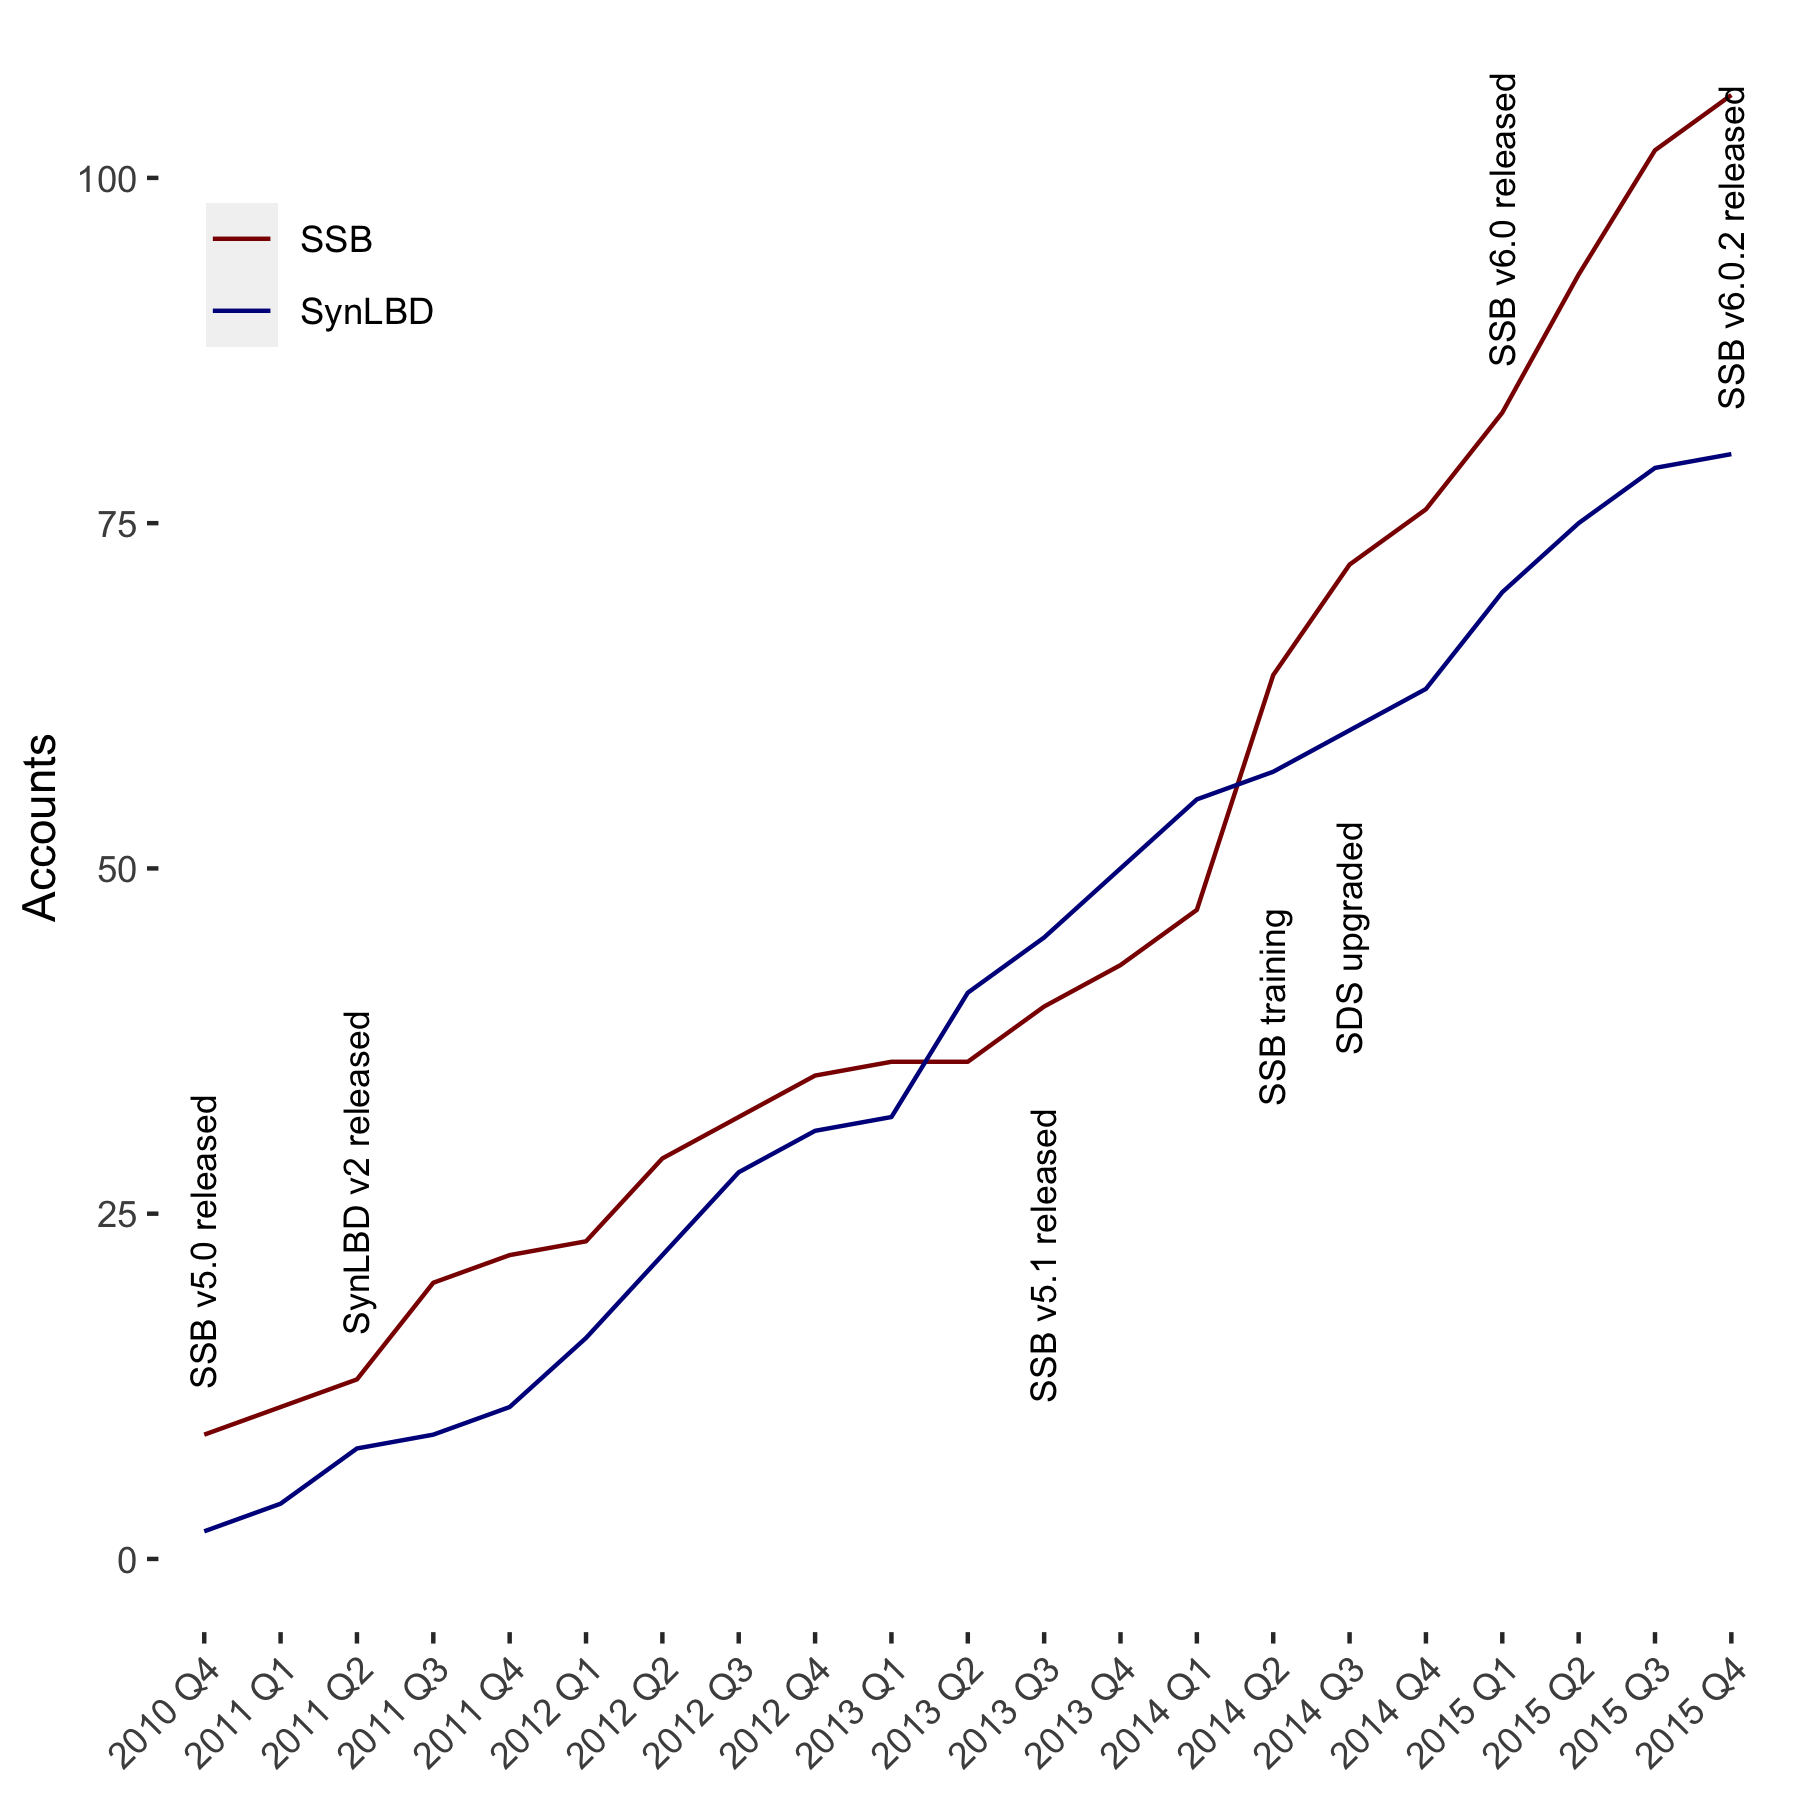
\includegraphics[height=0.8\textheight]{../../outputs/accounts-2015}
\end{center}
\footnotesize Growth substantially decreased afterwards: as of November 2022, about \textbf{160 users of SSB}, of which \textbf{22 active in the past year}.
\end{frame}


%%%%%%%%%%%%%%%%%%%%%%%%%%%%%%%%%%%%%%%%%%%%%%%%%%%%%%%%%%%%%%%%%%%%%%%%%%%%%%%
%%% defining the workflow picture: parameters
\definecolor{public}{RGB}{204,229,255}
\definecolor{restricted}{RGB}{255,153,153}
\definecolor{published}{RGB}{151,208,119}

\tikzstyle{decision} = [diamond, draw, 
                    fill=red!20, 
                    text width=4.5em, text badly centered, 
                    node distance=3cm, inner sep=0pt]
\tikzstyle{block} = [rectangle, draw, 
                    fill=green!20, 
                    text width=5em, text centered, 
                    rounded corners, minimum height=4em]
\tikzstyle{legend} = [rectangle, draw, 
                    text width=5.5em, text centered, 
                    dashed , minimum height=2em]
\tikzstyle{line} = [draw, -latex']
\tikzstyle{cloud} = [draw, ellipse,
                    fill=yellow!20, 
                    node distance=3cm,
                    minimum height=2em]
%%%%%%%%%%%%%%%%%%%%%%%%%%%%%%%%%%%%%%%%%%%%%%%%%%%%%%%%%%%%%%%%%%%%%%%%%%%%%%%
\newcommand{\blockdef}{%
\node [block,fill=white] (init) {request access SDS};
	\node [block, right of=init, node distance=3cm,fill=public] (develop) {develop model};
	\node [cloud, left of=init,fill=public] (researcher) {researcher};
	\node [block, below of=develop,fill=public] (submit) {submit code};
	\node [block, below of=submit, node distance=2.5cm,fill=public] (reproSDS) {reproduce on synthetic data};
	\node [cloud, right of=submit] (system) {NSI analyst};
	\node [block, right of=reproSDS, node distance=3cm,fill=restricted] (reproConf) {reproduce on confidential data};
	\node [decision, below of=reproConf,fill=restricted] (decide) {disclosure analysis};
    \node [block,left of=decide,node distance=9cm,fill=published] (publication) {publish results};
	\node [cloud, right of=decide, , align=center, node distance=4cm] (drb) {NSI disclosure \\ review board};
	
	\node [legend,below of=decide,fill=restricted] (legendConf) {secure area};
	\node [legend,left of=legendConf,fill=public,node distance=3cm] (legendPublic) {public area};
 }
\newcommand{\myworkflow}{%
	\begin{tikzpicture}[node distance = 2cm, auto]
	% Place nodes
	\blockdef{}
	% Draw edges
	\path [line] (init) -- (develop);
	\path [line] (develop) -- (submit);
	\path [line] (submit) -- (reproSDS);
	\path [line] (reproSDS) -- (reproConf);
	\path [line] (decide) --  (publication);
	\path [line] (reproConf) -- (decide);
	\path [line,dashed] (researcher) -- (init);
	\path [line,dashed] (system) -- (reproSDS);
	\path [line,dashed] (system) -- (reproConf);
	\path [line,dashed] (drb) -- (decide);
	\end{tikzpicture}
} % end command definition
\newcommand{\myworkflownon}{%
	\begin{tikzpicture}[node distance = 2cm, auto]
	% Place nodes
	\blockdef{}
    % override
    \node [block, below of=submit, node distance=2.5cm,fill=white] (reproSDS) {reproduce on synthetic data};
	% Draw edges
	\path [line] (init) -- (develop);
	\path [line] (develop) -- (submit);
	\path [line] (submit) -- (reproConf);
	\path [line] (decide) --  (publication);
	\path [line] (reproConf) -- (decide);
	\path [line,dashed] (researcher) -- (init);
	\path [line,dashed] (system) -- (reproConf);
	\path [line,dashed] (drb) -- (decide);
	\end{tikzpicture}
} % end command definition
\newcommand{\obtainingresults}{%
\begin{tikzpicture}[node distance = 2cm, auto]
	% Place nodes
	\node [block, fill=restricted] (reproConf) {reproduce on confidential data};
    \node [decision, below of=reproConf, fill=restricted] (decide) {disclosure analysis};
    \node [cloud, right of=decide, , align=center, node distance=4cm] (drb) {NSI disclosure \\ review board};
    % Draw edges
\path [line] (decide) -| node [near start] {results } (researcher);
\path [line] (reproConf) -- (decide);
\path [line,dashed] (drb) -- (decide);
	\end{tikzpicture}
 }
%%%%%%%%%%%%%%%%
\newcommand{\flowvalidation}{%
	\begin{tikzpicture}[node distance = 2cm, auto]
	% Place nodes
	\node [block, fill=public] (submit) {submit code};
	\node [block, fill=public, below of=submit, node distance=2.5cm] (reproSDS) {reproduce on synthetic data};
    \node [block, fill=restricted, right of=reproSDS, node distance=3cm] (reproConf) {reproduce on confidential data};
	\path [line] (submit) -- (reproSDS);
    \path [line] (reproSDS) -- (reproConf);
	\end{tikzpicture}
 }

 
\subsection{Workflow with Validation Server}

\begin{frame}
\frametitle{Workflow with Validation Server}

\scalebox{0.6}{
\myworkflow
}
\end{frame}

\begin{frame}
\frametitle{Workflow with Validation Server: In practice}

\scalebox{0.6}{
\myworkflownon
}
\end{frame}



\subsection{Access}

\begin{frame}{Access process}
\scalebox{0.1}{\myworkflow}
\scalebox{0.6}{
	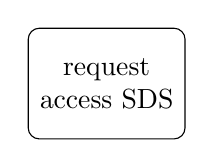
\begin{tikzpicture}[node distance = 2cm, auto]
	% Place nodes
	\node [block,fill=white] (init) {request access SDS};
	\end{tikzpicture}
}
\begin{block}{Simple access requests}
\begin{itemize}
	\item Access requests were sent to data custodians (separately for SynLBD and SSB)
	\item Access requests were only reviewed for feasibility (of the analysis on confidential data), but were not otherwise restricted. 
	\item Once access was verified,  the server provider (Cornell University) set up accounts on the system
	\end{itemize}
\end{block}
\end{frame}

%\begin{frame}{Access}
%\begin{block}{Server access}
%\begin{itemize}
%	\item Users gain access to a remote graphical desktop interface (Linux desktop,  \href{http://www.nomachine.com}{NX technology}).
%\end{itemize}
%\end{block}
%\end{frame}

\begin{frame}{Model Development}
	\scalebox{0.1}{\myworkflow}
	\scalebox{0.6}{
		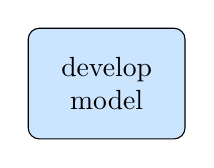
\begin{tikzpicture}[node distance = 2cm, auto]
			% Place nodes
			\node [block,fill=public] (develop) {develop model};
		\end{tikzpicture}
	}
	\begin{block}{Researchers work from their own offices $+$}
		\begin{itemize}
			\item No need to travel
			\item Low to zero cost
			\item Access to system and software at no charge
			\item No restrictions on type of model to be estimated
            \item Upload of files is moderated (enforce data provenance documentation, reproducibility, necessary for target environment)
		\end{itemize}
	\end{block}
	
\end{frame}




\begin{frame}{Validation}
\scalebox{0.1}{\myworkflow}
\scalebox{0.6}{
\flowvalidation{}
}

\begin{block}{Requirements}
\begin{itemize}
			\item all programs and auxiliary input files, 
			\item documentation of the results similar to a		{\it \color{orange}	disclosure review request at \ac{FSRDC}} , 
			\item all programs run error-free	(replicability requirement)
		\end{itemize}
\end{block}

\begin{block}{Process}
\begin{itemize}
			\item Conducted by program staff at Census Bureau
		\end{itemize}
\end{block}

\end{frame}





\begin{frame}{Obtaining results}
\scalebox{0.1}{\myworkflow}
\scalebox{0.6}{
	\obtainingresults{}
}
\begin{block}{Requirements}
\begin{itemize}
			\item documentation of the results similar to a		{\it \color{orange}	disclosure review request at \ac{FSRDC}} (assisted by program staff, no researcher interaction)
		\end{itemize}
\end{block}

\end{frame}


%%%%%%%%%%%%%%%%%%%%%%%%%%%%%%%%%%%%%%%%%%%%%%%%%%%%%% OUTCOMES







\section{Outcomes}

\subsection{Usage}

\begin{frame}{Accounts created (as of 2015)}
	\begin{center}
		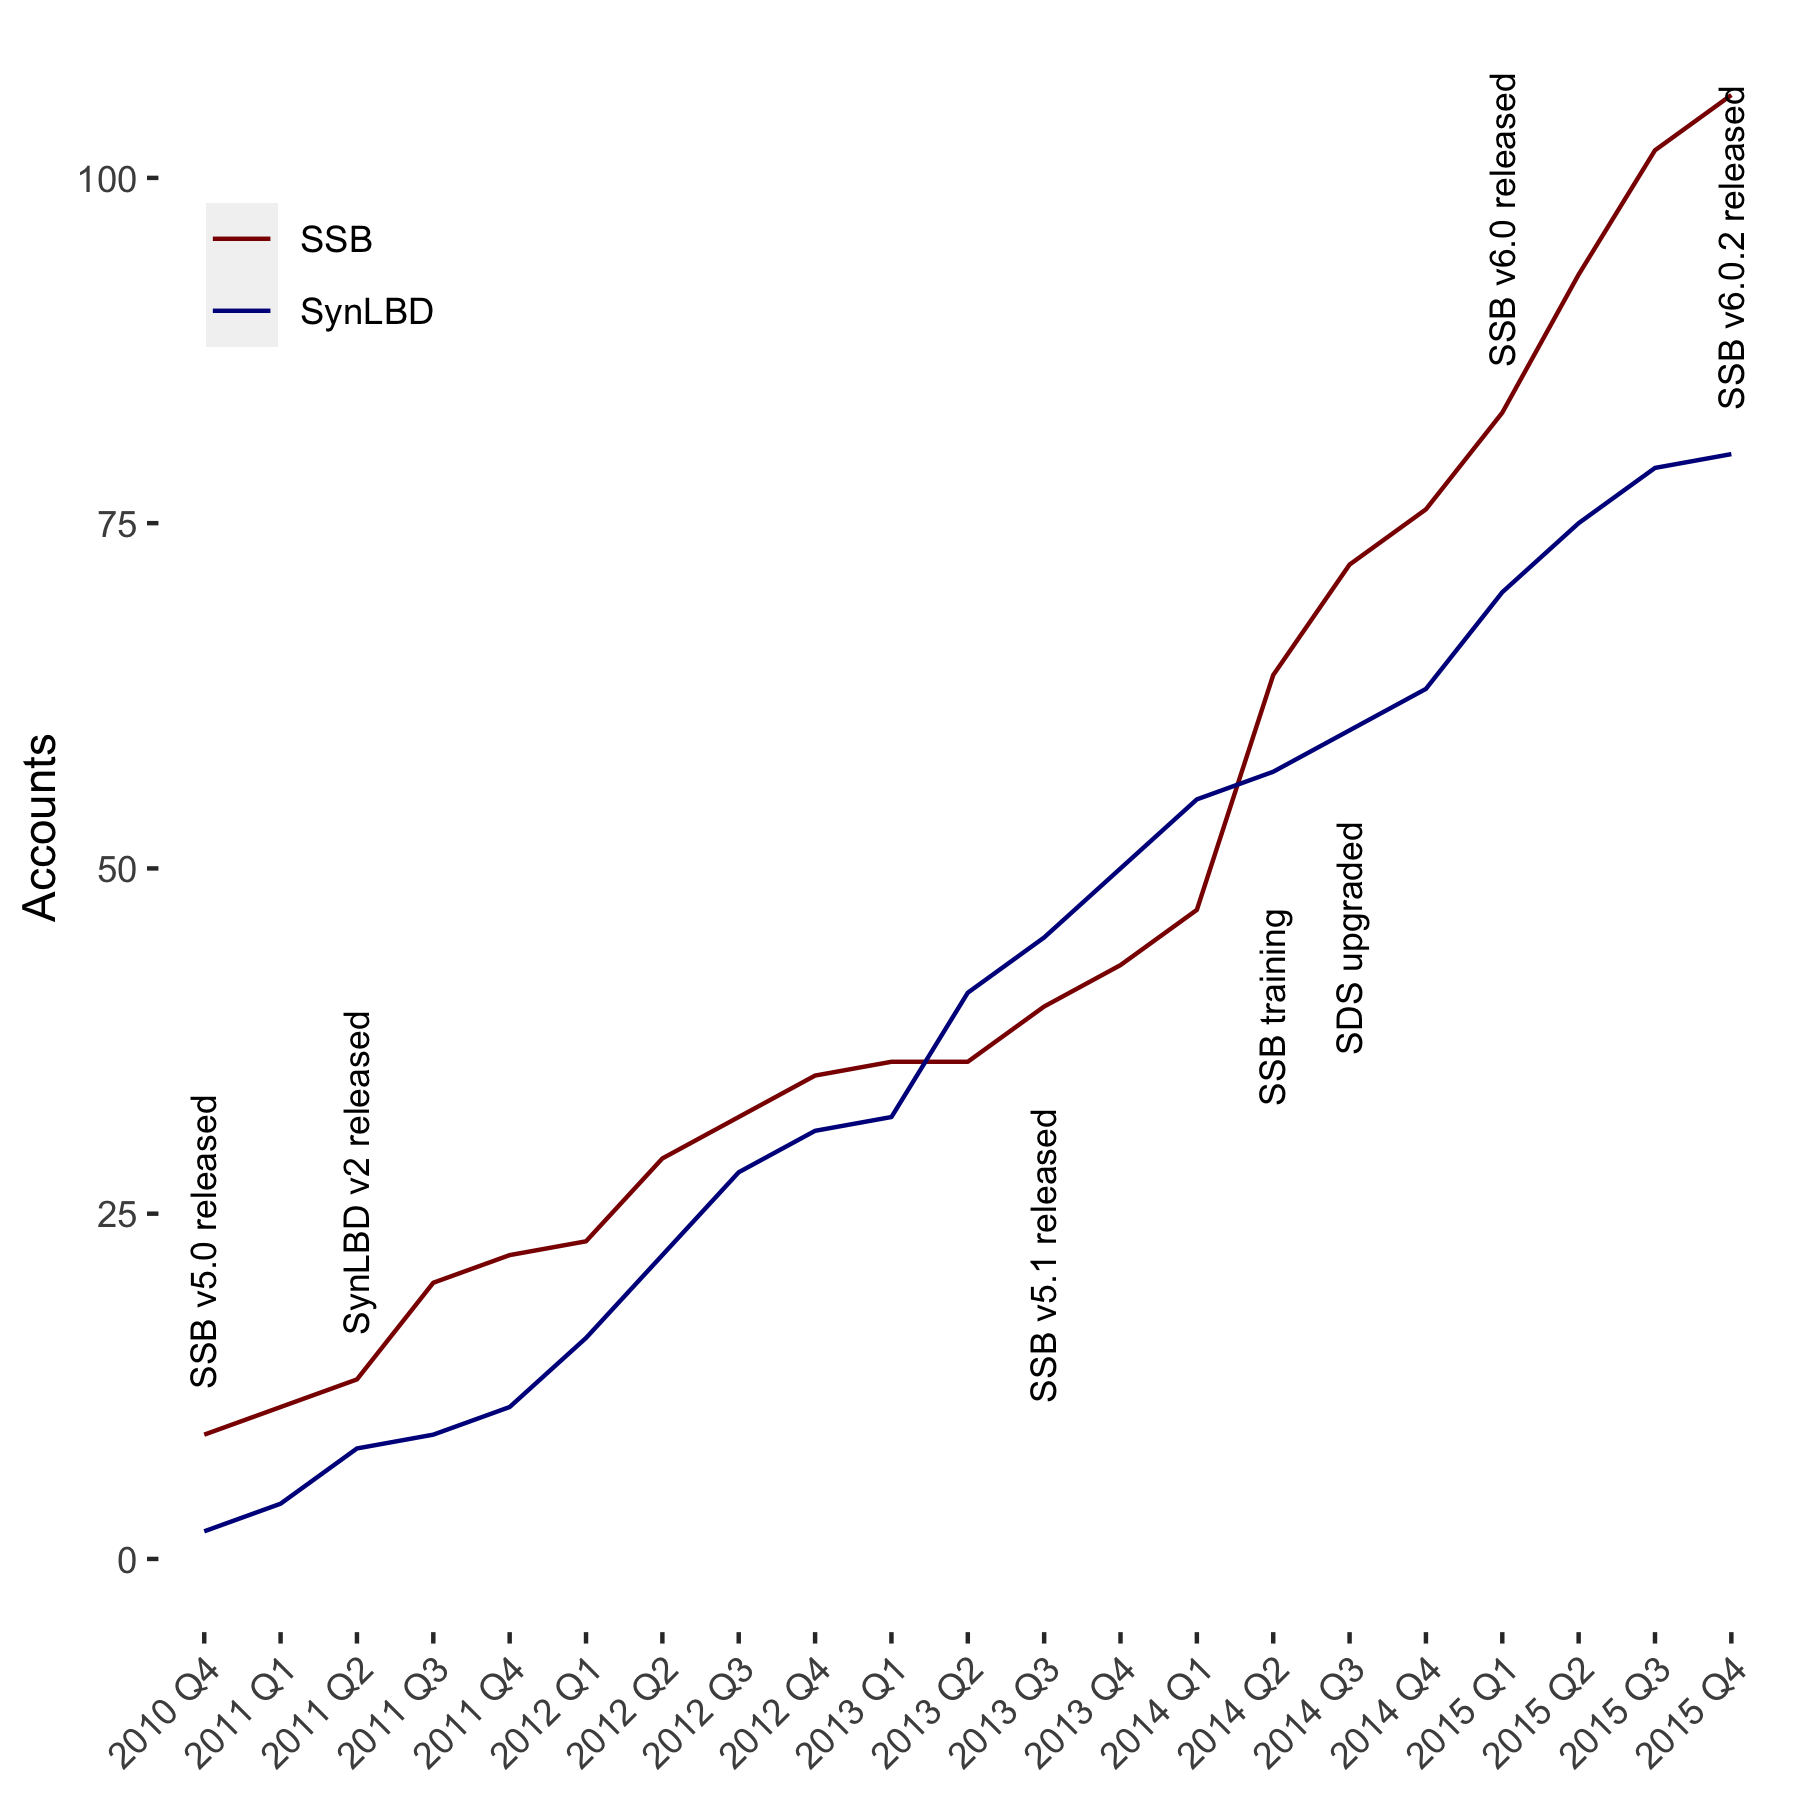
\includegraphics[height=0.8\textheight]{../../outputs/accounts-2015}
	\end{center}
\end{frame}


%
%\begin{frame}{Accounts created}
%	\begin{itemize}
%		\item As of 2015 Q4, 186 accounts created
%		\item Surges when presentations or training are held
%	\end{itemize}
%\end{frame}



\begin{frame}{Analysis of denied applications: Feasibility}
\begin{figure}[h]
	\Tree[.{SynLBD applications as of 2017 (100)} 
	[.{Accepted (79)}
	]
	%%%%%%%%%
	[.{Denied (21)}
	[. {Firm vars (6)} {Geo vars (11)} {NAICS (1)}
	]  ]
	]
%	\caption{A Breakdown of the Articles\label{tree}}
\end{figure}
\tiny Based on analysis of universe of applications as of 2017.
\end{frame}



\begin{frame}{Key feature: Feedback loop}
User feedback (also survey) incorporated into each version
\begin{block}{SSB}
\begin{itemize}
	\item Variables
	\item Structure
\end{itemize}
$\rightarrow$ V5, V6, V7 (see \cite{CreationSSBv7} for details)
\end{block}
\begin{block}{SynLBD}
\begin{itemize}
	\item NAICS
	\item firm-structure
	\item geography 
\end{itemize}
$\rightarrow$ V3.0 (unreleased, see \cite{RePEc:cen:wpaper:14-12} for plans)
\end{block}	
\end{frame}



\subsection{Validation}


\begin{frame}{Validation}
\begin{block}{For both datasets}
about 8 out every 100 projects request validation
\end{block}
\end{frame}


\begin{frame}{An ideal example: Bertrand et al (2015)}
\begin{block}{\cite{Bertrand29012015}}
\begin{columns}
\begin{column}{.5\textwidth}
	\includegraphics[height=0.7\textheight]{../../outputs/Bertrand-QJE-2015-FigureIII.png}
\end{column}
\begin{column}{.45\textwidth}
	There is a distinct break in the distribution of couples 
when the wife's income surpassed 50\% (their Figure~3)

\end{column}
\end{columns}\end{block}
\end{frame}


\begin{frame}{An ideal example: Bertrand et al (2015)}
%	\begin{block}{ SSB}
\begin{columns}
\begin{column}{.5\textwidth}
Bertrand et al on SSB

	\includegraphics[width=\textwidth]{../../outputs/jma_graph_rel_earn3_syn.png}\end{column}
\begin{column}{.5\textwidth}
	%\pause
	\only<1>{No such break in the synthetic data}
	 \only<2>{\cite{Bertrand29012015}:
	 	
	 	\includegraphics[width=\textwidth]{../../outputs/jma_graph_rel_earn3.png}}
\end{column} 
\end{columns}

%\end{block}
\end{frame}

\begin{frame}{Analytic validity}
\begin{block}{General approach: \emph{proximity of coefficients} $
t_{\Delta \beta_{k,m}}$}

We compute
$$
t_{\Delta \beta_{k,m}} = \frac{\beta_{k,m} - \beta_{k,m}^*}{\sqrt{s_{k,m}^2 + s_{k,m}^{*2}}}
$$
and assess its statistical significance (90\% bilateral). The \textbf{higher} the fraction of \textbf{insignificant} tests across all estimated models and parameters, the closer the synthetic and confidential models are under the estimated models.
\end{block}
\end{frame}

\begin{frame}{Analytic validity, more generally}
\begin{block}{General approach: \emph{interval 
			overlap measure} $J_k$}
 \citep{tas2006} 
	
	Consider the overlap of \textbf{confidence intervals} for variable $n$
\begin{columns}
	\begin{column}{0.5\textwidth}
	\begin{itemize}[<+->]
		\item $(L,U)$ for $\beta_n$ (from the confidential data ) 
		\item  $(L^{*},U^{*})$ for $\beta_n^*$ (from synthetic data)
	\item {Let $L^{over} = \max (L,L^{*} )$ and $U^{over} = \min (U,U^{*})$.}
	\end{itemize}
	\end{column}
\begin{column}{0.5\textwidth}
 \only<1>{\includegraphics[width=\textwidth]{../../outputs/overlap-1.png}}
 \only<2>{\includegraphics[width=\textwidth]{../../outputs/overlap-3.png}}
 \only<3>{\includegraphics[width=\textwidth]{../../outputs/overlap-4.png}}
\end{column}
\end{columns}
\end{block}
\end{frame}	
	
\begin{frame}{Analytic validity}
	\begin{block}{	Then the  overlap in confidence intervals is}

	
	$$
	J_k^{*} = \frac{1}{2} \left [ \frac{U^{over} - L^{over}}{U-L} + \frac{U^{over} - L^{over}}{U^*-L ^*}        \right ]
	$$
\end{block}
\end{frame}

\begin{frame}{Challenges in measurement}
	\begin{block}{No systematic mechanism implemented from the start}
		\begin{itemize}
			\item In collaboration with Census Bureau, we added code to users' SAS/Stata programs ex-post, attempting to capture parameter values estimated
			\item \textbf{Difficult}, because no homogeneous structure 
			\item \textbf{Limiting}, since no easy way to identify ``main parameters'' of interest from ``nuissance'' parameters (controls)
		\end{itemize}
	\end{block}
\end{frame}

\begin{frame}{Analytic validity}
	\begin{block}{Proximity $
			t_{\Delta \beta_{k,m}}$}
		\centering
		\input{../table_proximity}
	\end{block}
\footnotesize Fraction of test statistics that are not significant. Higher is better.
\end{frame}

\begin{frame}{Analytic validity}
\begin{block}{Coverage $J_k^{*}$}
	\centering
\input{../table_coverage}
\end{block}
\footnotesize Distribution of coverage across all parameters. Higher is better.
\end{frame}

	
	

\begin{frame}{Gateway data}
\begin{figure}
	\centering
	\caption{Connection between Census RDC usage and Synthetic Data Server}\label{fig:rdcUse}
	\includegraphics[height=0.6\textheight]{../../outputs/useRDCgraph.png}
\end{figure}
\footnotesize Based on a manual analysis of (FS)RDC projects in 2017.
\end{frame}
 

\begin{frame}{SDS and FSRDC}
\begin{block}{Other outcomes/interactions}
\begin{itemize}
	\item at least some of the RDC projects were
direct continuation of SDS projects%, in domains that were not covered by the synthetic data, but the analysis for which was prepared for on the SDS. 
 (source: private conversations)
	\item average delay (project start (SDS), project start (RDC)) : 400 days.
	\item (reminder:  turnaround for validation = [ 7, 90 ]  days...)
\end{itemize}
\end{block}
\end{frame}



%%%%%%%%%%%%%%%%%%%%%%%%%%%%%%%%%%%%%%%%%%%%%%%%%%%%%% LESSONS


\section{Lessons}

\begin{frame}{Lessons}
\vfill
    \begin{block}{Some Lessons Learned from the Pilot}
        
    \end{block}
    \vfill
    \hfill \tiny \color{gray} [\hyperlink{sec:pilot:summary}{TLDR}]
\end{frame}

\subsection{Access}

\begin{frame}{Access process}
\scalebox{0.1}{\myworkflow}
\scalebox{0.6}{
	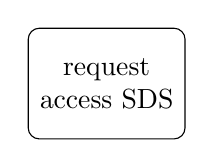
\begin{tikzpicture}[node distance = 2cm, auto]
	% Place nodes
	\node [block,fill=white] (init) {request access SDS};
	\end{tikzpicture}
}
\begin{block}{Access requests}
\begin{itemize}
	\item \textbf{Manual} process
	\item Simple, when compared to access to FSRDC
	\item Typical turnaround time is \textbf{1-10 days}
\end{itemize}
\tiny Not homogeneous across datasets
\end{block}
\end{frame}

%\begin{frame}{Access}
%\begin{block}{Server access}
%\begin{itemize}
%	\item Users gain access to a remote graphical desktop interface (Linux desktop,  \href{http://www.nomachine.com}{NX technology}).
%\end{itemize}
%\end{block}
%\end{frame}

\subsection{Model Development}

\begin{frame}{Model Development}
\scalebox{0.1}{\myworkflow}
\scalebox{0.6}{
	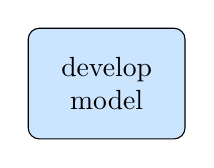
\begin{tikzpicture}[node distance = 2cm, auto]
	% Place nodes
	\node [block, fill=public] (develop) {develop model};
	\end{tikzpicture}
}
\begin{block}{Challenges/ Lessons for Researchers}
	\begin{itemize}
		\item do not work in their \textbf{usual} work environment ({\it \color{orange} perceived or real lack of flexibility})
		\item must incorporate future disclosure avoidance requirements into their analysis (note: {\it\color{orange}little guidance, no tools})
		\item must avoid hard-coded (data-informed) programming, and use data-dependent (automated) code (this seems {\it \color{orange} challenging for many researchers})
		\item develop code interactively, but must ultimately submit to an (semi-) automated system ({\it \color{orange} = reproducibility, not always clearly communicated})
	\end{itemize}
	\end{block}
\end{frame}



\begin{frame}{Model Development}
\scalebox{0.1}{\myworkflow}
\scalebox{0.6}{
	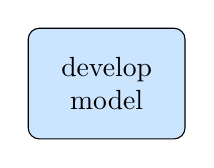
\begin{tikzpicture}[node distance = 2cm, auto]
	% Place nodes
	\node [block, fill=public] (develop) {develop model};
	\end{tikzpicture}
}
\begin{block}{Server transfers}
	\begin{itemize}
		\item Requests for removal of \textit{results} are \textit{\color{orange} \textbf{manually} moderated} - \textbf{take a few days}
		\item  {\it \color{orange}Upload requests for auxiliary data are \textbf{manually} moderated} 
	\end{itemize}
\end{block}\pause

\begin{block}{Server access}
	\begin{itemize}
		\item software is limited to \textbf{SAS, Stata}. 
		\item R, Matlab, Python may be available upon special request and upon coordination with data custodians ({\it \color{orange}limitation imposed by target environment}, mostly accomodated). 
	\end{itemize}
\end{block}
\end{frame}



\subsection{Validation}

\begin{frame}{Validation}
\scalebox{0.1}{\myworkflow}
\scalebox{0.6}{
\flowvalidation{}
}

\begin{block}{Challenges}
	\begin{itemize}
		\item Anecdotally, code often fails upon first validation attempt  
		\item Not automated (submission, feedback, reproduction), involves {\it \bf \color{orange}(lots of) manual labor}
	\end{itemize}
\end{block}

\end{frame}


\subsection{Validation}


\begin{frame}{Obtaining results}
\scalebox{0.1}{\myworkflow}
\scalebox{0.6}{
	\obtainingresults{}
}

\begin{block}{Challenges}
\begin{itemize}
	\item Validated results must \textbf{\color{orange}pass disclosure-avoidance analysis} $\rightarrow$ some limitation (quantity, count restrictions) 
	\item requires that 	users provide  documentation of the results similar to a {\it \color{orange}	disclosure review request at \ac{FSRDC}} ({\bf \color{orange} Challenging, and these have evolved over time!}), 
	\item delays have increased ({\bf \color{orange}substantially!}) over time
	\end{itemize}
\end{block}
\end{frame}





\subsection{Summary of Pilot}
\label{sec:pilot:summary}

\begin{frame}{Some tentative conclusions}
\scalebox{0.1}{\myworkflow{}}
\begin{block}{Process}
\begin{itemize}
    \item Multiple friction points: Disclosure of results, Initial access, Development, Removal of results based on synthetic data (in decreasing order of importance)
    \item Due to nature of pilot, labor intensity is high (no automation)
    \item User support should be improved: Tools to prepare and assess disclosure avoidance measures, success of porting model
\end{itemize}
\end{block} 
\end{frame}



\begin{frame}{Some tentative conclusions}
%\scalebox{0.8}{
\includegraphics[width=0.3\textwidth]{../../outputs/overlap-cropped.png}
\begin{block}{Data and models}
\begin{itemize}
    \item In general, data quality is sufficient for model development
    \item In general, data quality is insufficient to replace confidential data!
    \item Almost no user published results based on synthetic data {\tiny (Exception: \citet{perla2021})}
    \item Even simple papers have over 100 parameters {\tiny (Ex. \citet{10.1257/pandp.20181050})}
\end{itemize}
\end{block}
    
\end{frame}



%%%%%%%%%%%%%%%%%%%%%%%%%%%%%%%%%%%%%%%%%%%%%%%%%%%
\section{Next steps}

\subsection{Goals}


\begin{frame}{Basic goals}
\begin{block}{Maintain general approach}
    \begin{itemize}
        \item Allow for arbitrary model development (subject to minimal constraints)
        \item Allow for broad software usage
    \end{itemize}
\end{block} 
\end{frame}

\begin{frame}{Basic Goals}
\begin{block}{Reduce  friction points}
    \begin{itemize}
        \item Streamlined and fast (minutes, not months) access to data, validation
        \item User-centered  development
        \item Integrated disclosure avoidance for validation
        \item Greater conformance of database schema
        \item Lower barriers of entry
    \end{itemize}
\end{block}
\end{frame}

\begin{frame}{Basic Goals}
\begin{block}{Reduce cost}
    \begin{itemize}
    \item Automation and self-checks
        \item User-hosted development 
        \item Lower analytic validity of the synthetic data, easier confidentiality protection
    \end{itemize}
\end{block} 
\end{frame}


\subsection{Details}


\begin{frame}{Lower analytic validity}
\begin{block}{Trade-off}
    \begin{itemize}
        \item Reduce target analytic validity (limit target model coverage)
        \item Easier confidentiality protection enables easier access model
        \item Allows for full schema coverage (all variables present in confidential and synthetic data, with varying fidelity)
    \end{itemize}
\end{block}
    
\end{frame}

\begin{frame}{Data Access}
\begin{block}{Licensed access to synthetic data}
\begin{itemize}
    \item Provide licensed access to the synthetic data.
    \item Data can be downloaded to arbitrary system, subject to recorded license agreement \textit{[analog: IPUMS]}
    \item License specifies the limitations of the data, acknowledgement by user \textit{[analog: MIT software license]}
\end{itemize}
\end{block}
Note: Emphasis that the synthetic data is \textbf{not analytically valid/robust} is key!
\end{frame}

\begin{frame}{Validation Access}
\begin{block}{Controlled access to validation}
\begin{itemize}
    \item Provide API for validation \textit{[analog: geocoding systems]}
    \item API requires simple sign-up, with acknowledgement of limitations \textit{[analog: IPUMS Beta, industry models]}
    \item API can be wrapped into software-specific packages \textit{[goal: ease of use]}
    \item Validation is \textbf{fully automated}! \textit{(Including disclosure avoidance)}
    \item \textbf{API can be used to verify reproducibility} of submitted packages prior to validation
\end{itemize}
\end{block}

\end{frame}


\begin{frame}[fragile]{Example of API}
\begin{block}{Simplify and Scale}
		New school
	\begin{verbatim}
	import validate from census_validation
	# test the analysis
	myanalysis.syntheticdata.output
	# validate the analysis
	validate.authenticate()
	myanalysis.validate.output
	\end{verbatim}
\end{block}
\end{frame}

% $M(\Xi(D)) = M(D^*) \rightarrow Y^*$
\begin{frame}{Validation Output}
\begin{block}{Blended outputs}
Combine outputs to reduce disclosure risk:
\begin{itemize}
    \item If  Verification \citep{reiterVerificationServersEnabling2009,barrientos2018a} is positive ($Q(Y,Y^*)>\overline{q}$), provide output from synthetic data {\color{blue} [$M(\Xi(D))=Y^*$]}
    \item If Verification fails, provide (partial?) output from validation against confidential data {\color{blue} [$\Xi(M(D)) = Y'$]}
    \item If quality of confidentialized output is too low ($Q(Y')<\overline{q}$), suppress and prepare FSRDC proposal...
\end{itemize}
\end{block}
\end{frame}


\begin{frame}{Conditions for success}
\begin{block}{Reproducibility of code}
It is crucial that submitted code be reproducible. 
\end{block}
\begin{block}{Automation of disclosure avoidance}
Disclosure avoidance tools must be built in (easy to verify without manual intervention, prior to submission)
\begin{itemize}
    \item Set expectations
    \item Streamline / speed-up result release
\end{itemize}
\end{block}
\end{frame}


\subsection{Example}
\begin{frame}{Example}
\begin{block}{Containerized processing}
    \includegraphics[width=0.5\textwidth]{../../screenshots/gh-codeview.png}
    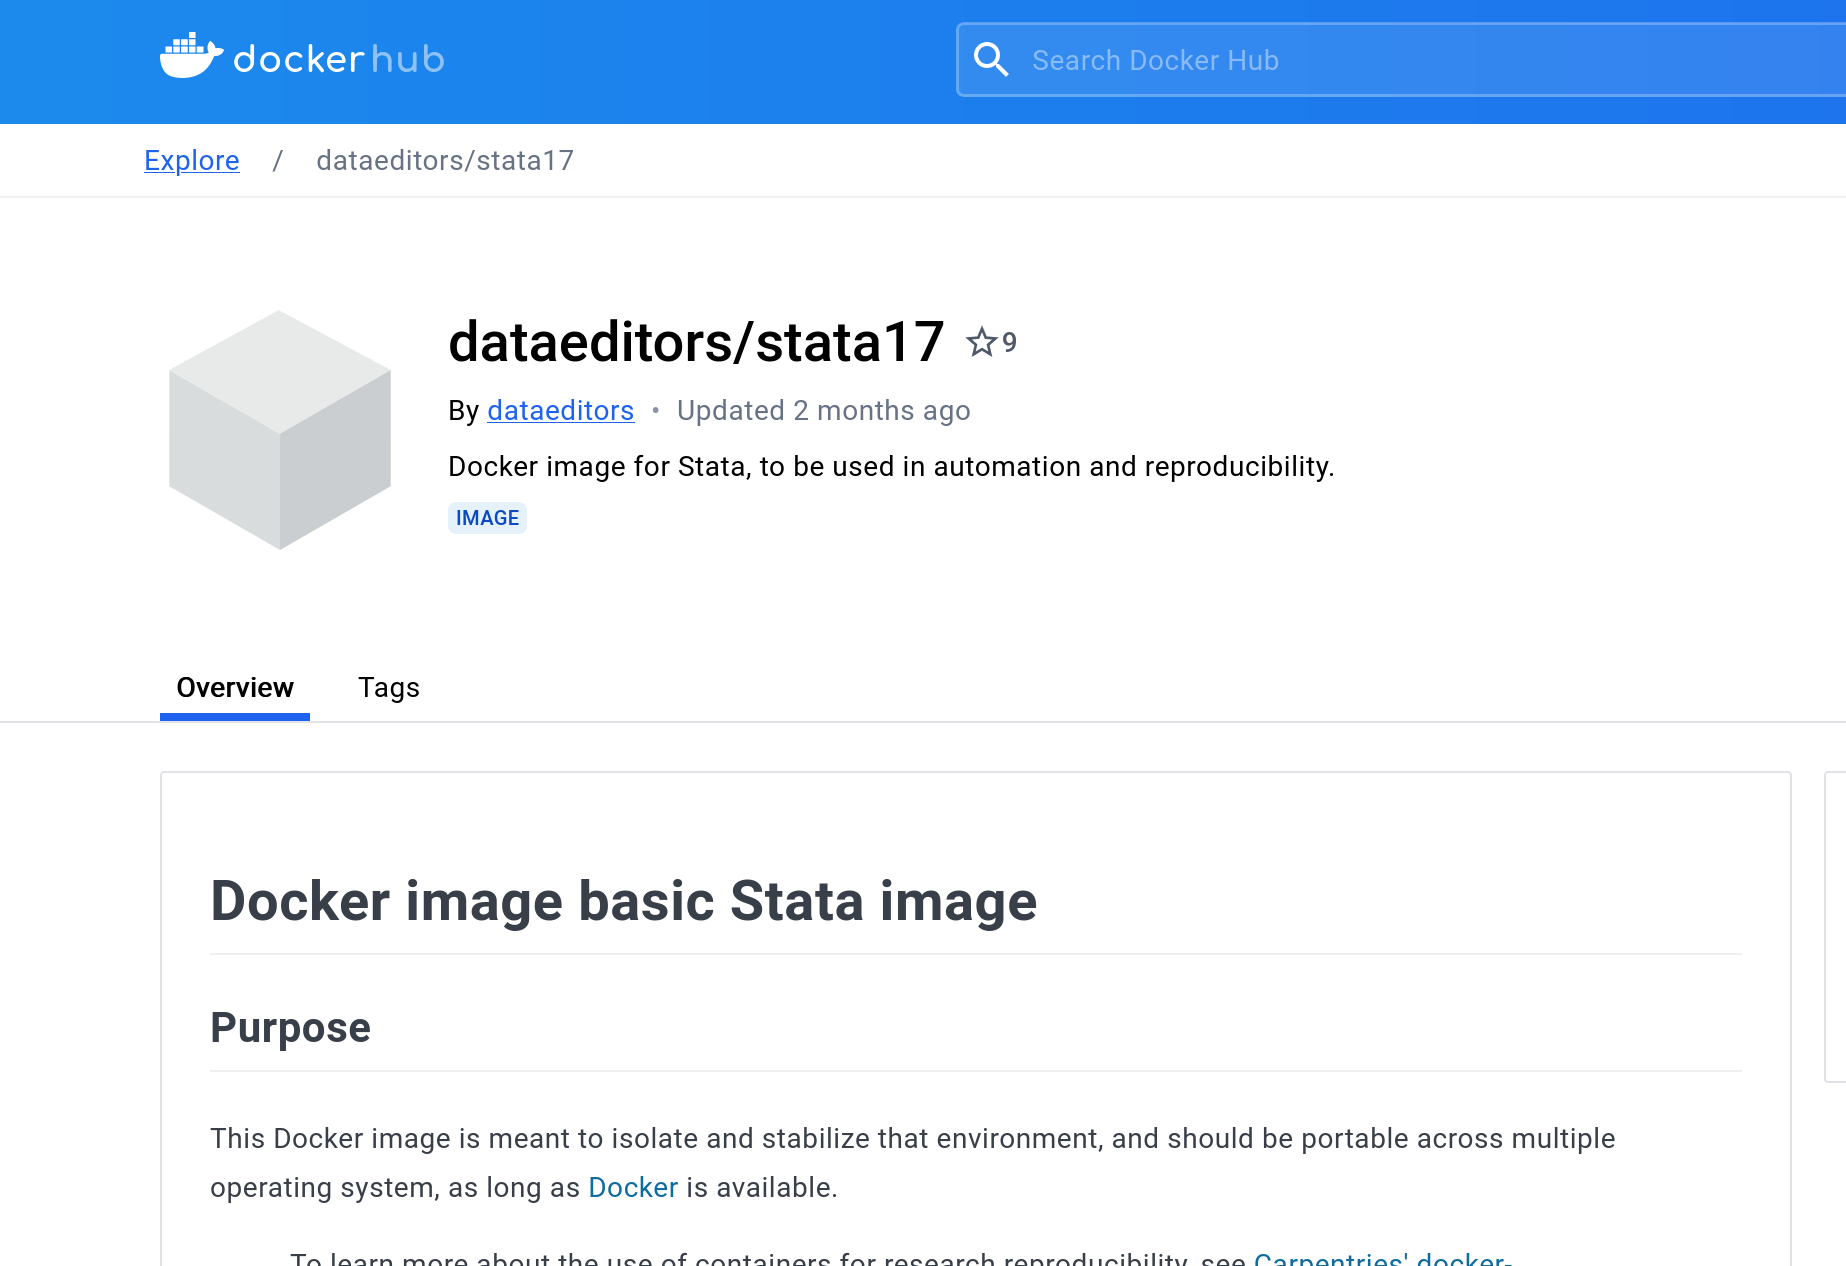
\includegraphics[width=0.45\textwidth]{../../screenshots/dockerhub-stata17.png}
\end{block}
\end{frame}

\begin{frame}{Example}
\begin{block}{Container can be run on author's computer}
  \centering  \includegraphics[height=0.7\textheight]{../../screenshots/local-docker.png}
\end{block}
\end{frame}

\begin{frame}[fragile]{Example}
\begin{block}{Validating reproducibility}
Run code non-interactively
	 {\footnotesize
	\begin{verbatim}
	docker run -it --rm --workdir /code \
       -v "$PWD/stata.lic":/usr/local/stata/stata.lic  \ 
       --volume "$PWD/data":/data        \
       --volume "$PWD/code":/code        \ 
       --volume "$PWD/results":/results  \
       69da7c49-f71b-4d08-918e-6cdccd8cd4c2 \
       \
       \
       /usr/local/stata/stata-mp analysis.do

	\end{verbatim}
 }
\end{block}
\end{frame}


\begin{frame}[fragile]{Example}
\begin{block}{Submitting for validation}
	 {\footnotesize
	\begin{verbatim}
	docker run -it --rm \
       --volume "$PWD/data":/data        \
       --volume "$PWD/code":/code        \ 
       --volume "$PWD/results":/results  \
       69da7c49-f71b-4d08-918e-6cdccd8cd4c2 \
       \
       \
       /special/validate $APIKEY $myemail
	\end{verbatim}
 }
\end{block}
\end{frame}

\begin{frame}[fragile]{Example}
\begin{block}{Submitting for validation}
	 {\footnotesize
	\begin{verbatim}
	trace submit --validate .
	\end{verbatim}
 }
\end{block}
\end{frame}

\begin{frame}[fragile]{Example}
\begin{block}{Validation}
	 {\footnotesize
	\begin{verbatim}
	docker run -it --rm \
       --volume "/path/to/confidential/data":/data       <======= \
       --volume "$PWD/code":/code        \ 
       --volume "$PWD/results":/results  \
       69da7c49-f71b-4d08-918e-6cdccd8cd4c2 \
       \
       \
       /usr/local/stata/stata-mp analysis.do
	\end{verbatim}
 }
\end{block}
\end{frame}



\begin{frame}{Science fiction?}
\begin{block}{All but one exist}
\texttt{/special/validate} does not exist yet.
\end{block}
\end{frame}

\begin{frame}{Security?}
\begin{block}{Isolation can be brought to bear}
Containerization not per-se security software, but only clear-text data transmitted
\end{block}
\includegraphics[height=0.25\textheight]{../../screenshots/gh-Dockerfile.png}
\end{frame}



\begin{frame}{Cannot install Docker?}
\begin{center}
    NOTE: Not an endorsement.
\end{center}
    \begin{block}{Use cloud service}
        \begin{itemize}
            \item AWS, Google Cloud, Azure, Github Codespaces
            \item (free or low-cost: pennies per compute hour)
        \end{itemize}
    \end{block}
\includegraphics[width=0.4\textwidth]{../../screenshots/gh-codeview.png}
\includegraphics[width=0.4\textwidth]{../../screenshots/gh-cs-stata.png}
\end{frame}



\begin{frame}{Not user friendly?}
    \begin{block}{Correct}
        \begin{itemize}
            \item Could be integrated into software packages (\texttt{ssc install censusvalidate} or \texttt{install.packages("censusvalidate")})
            \item Use existing online systems (free or low-cost)
        \end{itemize}
    \end{block}
\end{frame}

\begin{frame}{Using Commercial Services}
\begin{center}
    NOTE: Not an endorsement.
\end{center}
\includegraphics[height=0.4\textwidth]{../../screenshots/co-interface.png}
\end{frame}

\begin{frame}{Using Commercial Services}
\begin{center}
    NOTE: Not an endorsement.

\includegraphics[height=0.4\textwidth]{../../screenshots/co-logs.png}
\end{center}

\end{frame}



\section{Recommendations}
\begin{frame}{Recommendations}
	\begin{enumerate}
		\item Provide scalable mechanism - packages, API, submission websites, licensed data, etc.
		\item Provide clear disclosure avoidance criteria and \textbf{tools}
		\item Provide set of results: Verification \citep{reiterVerificationServersEnabling2009,barrientos2018a}, validation, only then FSRDC 
		\item Provide fast turnaround time (minutes, not months)
	\end{enumerate}
\end{frame}


\begin{frame}{Current Barriers}
	\begin{enumerate}
		\item Provide scalable mechanism - packages, API, submission websites, licensed data, etc.
		\item {\color{orange} \bf Provide clear disclosure avoidance criteria and \textbf{tools}}
		\item Provide set of solutions: Verification \citep{reiterVerificationServersEnabling2009,barrientos2018a}, validation, only then FSRDC ({\color{orange} Statistics of this})
		\item Provide fast turnaround time (minutes, not months)
	\end{enumerate}
\end{frame}


\begin{frame}
	\vfill
	\centering
	\begin{beamercolorbox}[sep=8pt,center,shadow=true,rounded=true]{title}
		\usebeamerfont{title}Thank you!\par%
	\end{beamercolorbox}
	\vfill
\end{frame}






%%% Local Variables:
%%% mode: latex
%%% End:

